\subsection{Derived quantities} \label{subsec:DerivedQuantities}
The value of inductance, capacitance or resistance can be calculated once the impedance of the DUT is known, along with the dissipation and quality factor. This chapter will show how this can be achieved. Consider that in section \ref{sec:ImpedanceAnalysis} where the impedance of a DUT could be written in the rectangular form $Z = R \pm jX$. The $jX$ term represents the capacitive, or inductive, reactance that could be used to find the inductance or capacitance value of the DUT.

To find $jX$ is trivial and will be done only for a capacitor, the process for an inductor is the same. Consider the circuit on figure \refq{fig:4_1_1_CapCircuit} with a voltage source, $v(t)$, connected across a capacitor and a current $i(t)$ flowing in the circuit. 
\begin{figure}[H]
    \centering
    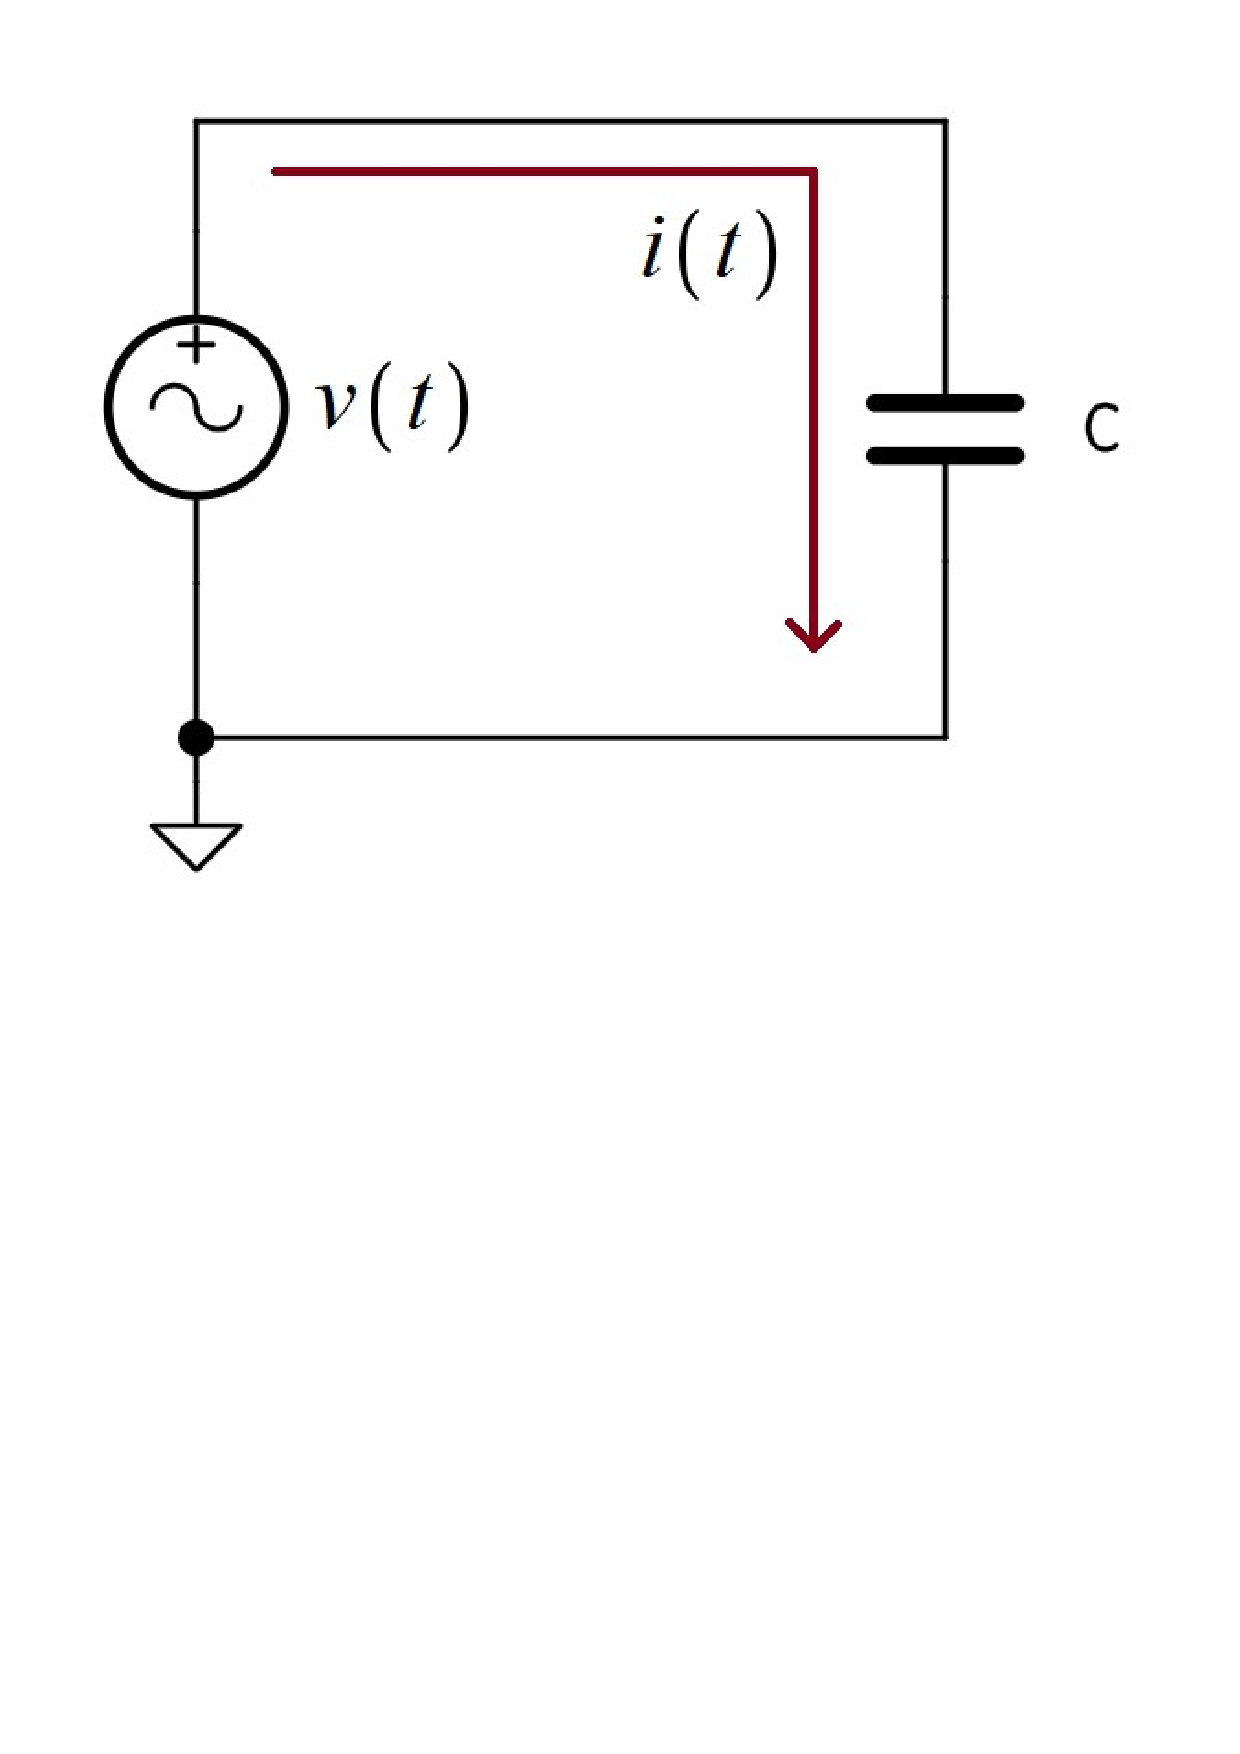
\includegraphics[clip, trim=0 400 0 0, width=0.60\textwidth]{Sections/4_TechnicalAnalysis/Figures/4_1_1_CapCircuit.pdf}
    \caption{An AC voltage source, $v(t)$, across a capacitor causes a current, $i(t)$, to flow through it.}
    \label{fig:4_1_1_CapCircuit}
\end{figure}

The current in the circuit is, because of the capacitor, as in eq \refq{eq:4_1_1_CapCurrent}.
\begin{equation}\label{eq:4_1_1_CapCurrent}
    i(t) = C\cdot\frac{d}{dt} (v(t))
\end{equation}
Transforming \refq{eq:4_1_1_CapCurrent} into the frequency domain with the laplace transform gives eq \refq{eq:4_1_1_CapCurrent2}.
\begin{equation}\label{eq:4_1_1_CapCurrent2}
    \Laplace\{\/i(t)\}\ = \Laplace\{\/C\cdot\frac{d}{dt} (v(t))\} \rightarrow I(s) = C\cdot(sV(s) - v(t=0^-))
\end{equation}
The circuit is supplied by an AC source and it is assumed that the circuit has reached a steady-state so that the initial condition of the voltage source is $v(t=0^-) = 0$. Solving for the reactance of the circuit $V(s) / I(s)$ gives eq \refq{eq:4_1_1_CapCurrent3}.
\begin{equation}\label{eq:4_1_1_CapCurrent3}
    \frac{V(s)}{I(s)} =X_c(s)= \frac{1}{sC}
\end{equation}
Substituting the laplace variable $s$ with $s = 0 + j\omega$ gives eq \refq{eq:4_1_1_CapCurrent4}.
\begin{equation}\label{eq:4_1_1_CapCurrent4}
    X_c(\omega) = \frac{1}{j\omega C}=-\frac{j}{\omega C}
\end{equation}
Note that the complex laplace variable is defined as $s = \sigma + j\omega$. The real part $\sigma$ represents exponential growth. By assuming the circuit is in steady-state, there is no exponential growth so $\sigma = 0$. The impedance for a circuit dominated by a capacitance will have the form $Z = R -\frac{j}{\omega C}$ as shown in eq \refq{eq:4_1_1_CapCurrent4}.

The value of capacitance can be found with eq \refq{eq:4_1_1_CapCurrent4} by just solving for C. This gives the phasor in eq \ref{eq:4_1_1_CapCurrent5}
\begin{equation}\label{eq:4_1_1_CapCurrent5}
    C(\omega)=-\frac{j}{X_C\cdot \omega}
\end{equation}
The quantity of interest at this point is the magnitude of capacitance as shown in eq \refq{eq:4_1_1_CapCurrent6}.
\begin{equation}\label{eq:4_1_1_CapCurrent6}
    |C(\omega)|= \sqrt{\left(-\frac{1}{X_C\cdot \omega}\right)^2} =\frac{1}{X_c\cdot \omega} 
\end{equation}

The result in eq \refq{eq:4_1_1_CapCurrent5} is obvious as the phasor in eq \refq{eq:4_1_1_CapCurrent5} is just pointing down the imaginary axis in the complex plane and thus has a magnitude of $abs(C)$. A similar exercise can be performed if the capacitor on figure \refq{fig:4_1_1_CapCircuit} was swapped with an inductor. The results is the expression for inductive reactance in eq \refq{eq:4_1_1_IndReactance}.
\begin{equation}\label{eq:4_1_1_IndReactance}
    X_l(\omega) = j \omega L
\end{equation}

Much like eq \refq{eq:4_1_1_CapCurrent6} the inductance value can be found with eq \refq{eq:4_1_1_IndReactance}. This is done in eq \refq{eq:4_1_1_IndReactance2}.

\begin{equation}\label{eq:4_1_1_IndReactance2}
    L(\omega) = \frac{X_l(\omega)}{j\omega} = -j\frac{X_l(\omega)}{\omega}
\end{equation}

Similar to eq \refq{eq:4_1_1_CapCurrent6} the magnitude of inductance is found and is as shown in eq \refq{eq:4_1_1_IndReactance3}.

\begin{equation}\label{eq:4_1_1_IndReactance3}
    |L(\omega)| = \sqrt{\left(-\frac{X_l(\omega)}{\omega}\right)^2} = \frac{X_l(\omega)}{\omega}
\end{equation}


Eq \refq{eq:4_1_1_CapCurrent6} and \refq{eq:4_1_1_IndReactance3} can be used to find the values of capacitance and inductance of the DUT. Real capacitors, and inductors, have undesired parasitic element like resistance in the materials used to make the components. This resistance is in series with the component and is dubbed the \textit{equivalent series resistance} (ESR) as shown on figure \refq{fig:4_1_1_CapESR} and is responsible for power dissipating as heat in the component.
\begin{figure}[H]
    \centering
    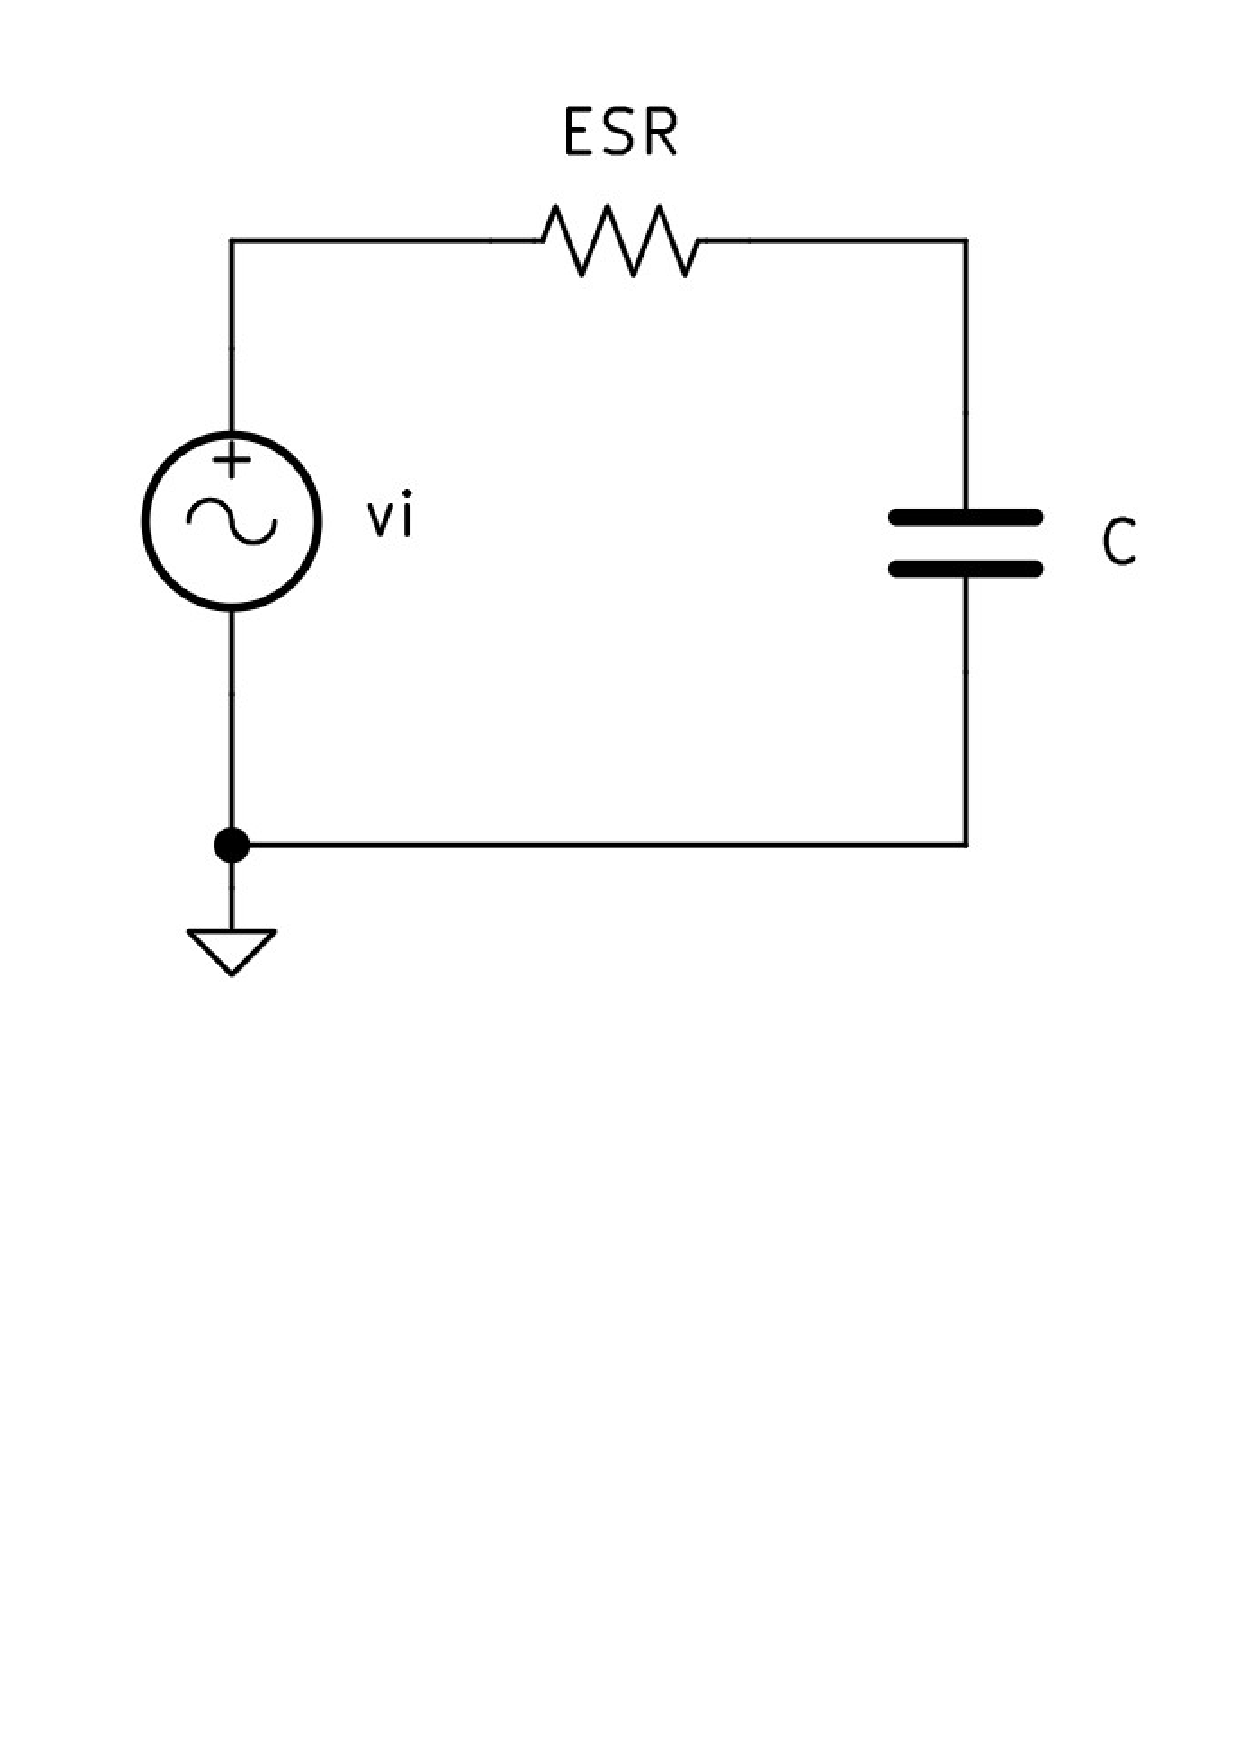
\includegraphics[clip, trim=0 350 0 0, width=0.4\textwidth]{Sections/4_TechnicalAnalysis/Figures/4_1_1_CapESR.pdf}
    \caption{The capacitor is not ideal. It has a finite amount of resistance in the materials it is made of.}
    \label{fig:4_1_1_CapESR}
\end{figure}

\textit{good} capacitors typically have a low ESR value while \textit{bad} capacitors have a high ESR value. 